\documentclass{article}
\usepackage{etoolbox}
\usepackage{tikz}
\usetikzlibrary{matrix}

\let\mystyle\empty
\newcommand{\populatestyle}{%
  \foreach \c [count=\i] in {red, green, blue} {
    \begingroup\edef\x{\endgroup
       \noexpand\gappto\noexpand\mystyle{column \i/.style={nodes={fill=\c}},}}\x
    }%
}
\populatestyle

\tikzset{mymatrix/.estyle={\mystyle}}

\begin{document}
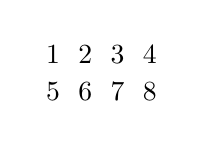
\begin{tikzpicture}
\matrix (m) [matrix of nodes,mymatrix] {
 1 & 2 & 3 & 4 \\
  5 & 6 & 7 & 8 \\ };
\end{tikzpicture}
\end{document}
